
\section{GROUP 18}
\begin{frame}
\frametitle{Overview group 18}
\begin{itemize}
\item Classification, $n\leq 5$
\item Statistical analysis of classification on a 5 $\times$ 5 grid
\item Algorithm for counting empty polygons
\item Idea!
\item executive summary
\end{itemize}
\end{frame}
% -----------------------------------------------------------------------


\begin{frame}
\frametitle{Classification $n=5$}
\begin{center}
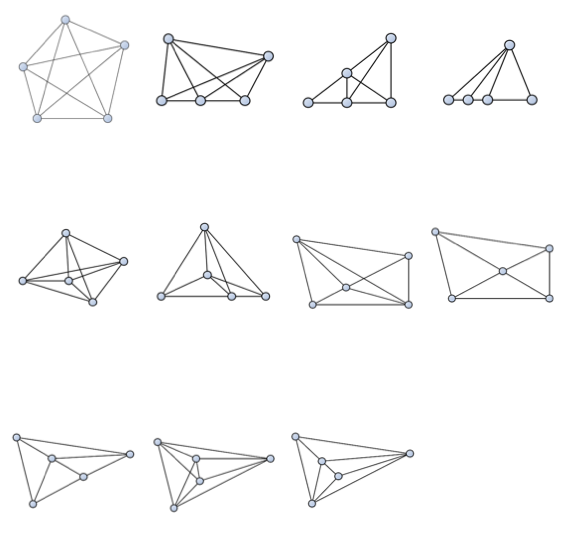
\includegraphics[width=8cm]{classification_overview.png}
\end{center}
\end{frame}
% -----------------------------------------------------------------------


\begin{frame}
\frametitle{5 point sets in a 5$\times$5 grid}
\begin{tabular}{l c r}
 class 5 (5-convex)                              &   11628   & 21,89 \% \\
 class 6 (5-convex, 1x collconvex)               &   13668   & 25,73 \%\\
 class 7 (5-convex, 2x collconvex)               &    1436   & 2,7 \% \\
 class 8 (5-convex, $>$2x collconvex)              &    1284 & 2,42 \% \\
 class 9 (4-convex)                              &   12800   & 24,1 \% \\
 class 10 (4-convex, 1xcollconvex)               &    2336   & 4,4 \% \\
 class 11 (4-convex, 1xcollinear)                &    6420   & 12,09 \% \\
 class 12 (4-convex, 2xcollinear)                &     578   & 1,09 \% \\
 class 13 (4-convex, 1xcollinear, 1x collconvex) &    1060   & 2 \% \\
 class 14 (3-convex)                             &     624   & 1,17 \% \\
 class 15 (3-convex, 1xcollconvex)               &    1284   & 2,42 \%
\end{tabular}
\end{frame}
% -----------------------------------------------------------------------


\begin{frame}
\frametitle{Algorithm for counting}
\begin{itemize}
\item first approach: for triangles brute force
\item tetragons:  recursive: deleting one point, inside-out test, count tetragon in $n-1$-gon 
\item problem: what if point is a collinear middlepoint?
\end{itemize}
\end{frame}
% -----------------------------------------------------------------------

\begin{frame}
\frametitle{}
\begin{itemize}
 \item Idea: our classification leads to number of polygons without calculating them
\end{itemize}
\end{frame}

% -----------------------------------------------------------------------

\begin{frame}
\frametitle{Webinterface}
 \begin{itemize}
  \item PHP-Webservice for other groups
  \item input: $n \leq 5$ Pointset on a $5 \times 5$ Grid
	\item output: classification and number of $n$-gons
	\item \url{http://www.upinthecloud.at/eca/getemptypolygons.php?pointset=0_0_2_1_4_0_2_2_2_4}
 \href{http://www.upinthecloud.at/eca/getemptypolygons.php?pointset=0_0_2_1_4_0_2_2_2_4}{\beamergotobutton{Link}}
 \end{itemize}
\end{frame}
% -----------------------------------------------------------------------


\begin{frame}
\frametitle{Webdemo for $5 \times 5$ Grid}
\begin{center}
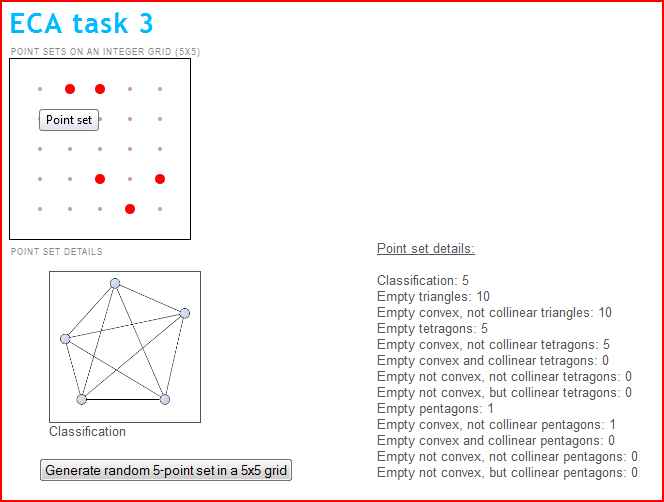
\includegraphics[width=9cm]{scshot.png}
\end{center}
 \begin{itemize}
  \item \url{http://www.upinthecloud.at/eca/ecatask3.html}
	  \href{http://www.upinthecloud.at/eca/ecatask3.html}{\beamergotobutton{Link}}
\end{itemize}
\end{frame}
% -----------------------------------------------------------------------

\begin{frame}
\frametitle{executive summary - group 18}
\begin{itemize}
\item Java tool for generating all pointsets for arbitrary grid size
\item Java classification tool for classifying and counting n-gons for a given pointset (arbitrary grid size)
\item JUnit tests for proof of concept
\item PHP-Webservice for classifying and counting n-gons for a given 5-pointset ($5\times 5$ grid)
\item Demo website for 5-pointsets on a $5\times 5$ grid
\end{itemize}
\end{frame}
% -----------------------------------------------------------------------


